\subsection{Motivation}

\begin{frame}{Recap: Motivation}
	\begin{mycolumns}[widths={50,50},animation=none]
		\myexampletight{Modularization of Cross-Cutting Concerns}{
			\centering
			\pic[width=1.0\linewidth]{aop-motivation-1}
		}
		\myexample{Feature Traceability}{
			find feature 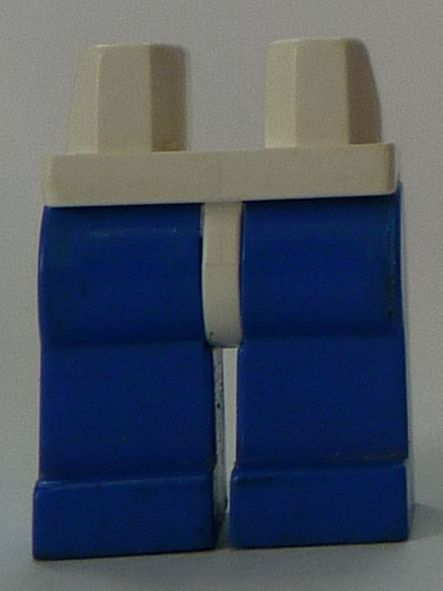
\includegraphics[width=.15\linewidth]{pants-blue} in product 
\includegraphics[width=.15\linewidth]{230}
		}
	\mynextcolumn
		\myexampletight{Flexible Extension / Minimal Preplanning}{
			\centering
			\pic[width=1.0\linewidth]{aop-motivation-2}
		}
		
		~
		
		\mynote{}{
			Achieving all this requires novel implementation techniques that overcome the limitations of classical object-oriented paradigms.
		}
	\end{mycolumns}
\end{frame}

\subsection{Aspects and Aspect Weaving}

\begin{frame}{Aspects and Aspect Weaving}
	\begin{mycolumns}[widths={50,50},animation=none]
		\mydefinition{Aspect \mysource{\fospl\mypages{143--145}}}{
			An aspect encapsulates the implementation of a crosscutting concern.
		}
		\mydefinition{Aspect Weaving \mysource{\fospl\mypages{143--145}}}{
			An aspect weaver merges the separate aspects of a program and the base program at user-selected program locations.
		}
		\mynote{}{
			\begin{itemize}
				\item Localizing a crosscutting concern within one code unit eliminates code scattering and tangling.
				\item An aspect can affect multiple other concerns with one piece of code, thereby avoiding code replication.
			\end{itemize}
		}
	\mynextcolumn
		\myexampletight{}{
			\centering
			\pic[width=1.0\linewidth]{aspect-weaving}
		}
	\end{mycolumns}
\end{frame}

\begin{frame}{Aspects and Aspect Weaving in Java: AspectJ}
	\begin{mycolumns}[widths={50,50},animation=none]
		\mydefinition{}{
			AspectJ is an aspect-oriented language extension of Java.
			\begin{itemize}
				\item Base program is written in Java (i.e., components = classes)
				\item Aspects are written in Java but typically include a multitute of new language constructs introduced by AspectJ
				\item Aspect weaver (aka.\ AspectJ Compiler) follows a compile-time binding approach (though certain decisions are made at runtime, s.\ later).
			\end{itemize}
		}
		\mynote{}{
			AspectJ is the most popular and widely used aspect-oriented language, all examples in this lecture will be given in AspectJ.
		}
	\mynextcolumn
		\myexampletight{}{
			\centering
			\pic[width=1.0\linewidth]{aspect-weaving}
		}
	\end{mycolumns}
\end{frame}

\subsection{Static vs. Dynamic Extensions}

\begin{frame}[fragile]{Static Extensions through Inter-Type Declarations}
	\begin{mycolumns}[widths={50,50},animation=none]
		\mydefinition{Inter-Type Declaration \mysource{\fospl\mypages{143--145}}}{
			An inter-type declaration injects a method, field, or interface from inside an aspect into an existing class or interface.
		}
		\mynote{Typical Usage}{
			Add field X / method Y to class Z
		}
	\mynextcolumn
\begin{codetight}{}
aspect Weighted {
	private int Edge.weight = 0;
	public void Edge.setWeight(int w) {
		weight = w;
	}
}
\end{codetight}
	\end{mycolumns}
\end{frame}

\begin{frame}{Dynamic Extensions through Join Points}
	\begin{mycolumns}[widths={50,50},animation=none]
		\mydefinition{Joint Point \mysource{\fospl\mypages{143--145}}}{
			A join point is an event in the execution of a program at which aspects can be woven into the program.
		}
		\mydefinition{Advice}{
			Code which is being executed when a join point matches. 
		}
		\mydefinition{Join-Points in AspectJ:}{
			\begin{itemize}
				\item Calling a method
				\item Execution of a method
				\item Access to a field (read or write)
				\item Catching an Exception
				\item Initialization of a class or object
				\item Execution of a Advice
				\item \ldots
			\end{itemize}
		}
	\mynextcolumn
		\myexampletight{}{
			\centering
			\pic[width=1.0\linewidth]{join_point_example}
		}
		\mynote{Open Question}{			
			How to specify the join points an aspect (i.e., an advice) affects?
		}
	\end{mycolumns}
\end{frame}

\subsection{Quantification}

\begin{frame}[fragile]{Quantification through Pointcuts}
	\begin{mycolumns}[widths={50,50},animation=none]
		\mydefinition{Pointcut \mysource{\fospl\mypages{143--145}}}{
			A pointcut is a declarative specification of the join points that an aspect affects. It is a predicate that determines whether a given join point matches.
		}
		\mydefinition{Quantification \mysource{\fospl\mypages{143--145}}}{
			Quantification is the process of selecting multiple join points based on a declarative specification (that is, based on a pointcut).
		}
		\myexample{}{
			\begin{itemize}
				\item Execute Advice X whenever the method setWeight of class Edge is called
				\item Execute Advice Y whenever any field in class Edge is accessed
				\item Execute Advice Z whenever a public method is called anywhere in the system and the method initialize has been called beforehand
			\end{itemize}
		}
	\mynextcolumn
\begin{codetight}{Anonymous Pointcut}
aspect A1 {
	after() : execution(int MathUtil.twice(int)) {
		System.out.println("MathUtil.twice executed");
	}
}
\end{codetight}			
\begin{codetight}{Explicit Pointcut}
aspect A2 {
	pointcut executeTwice() : execution(int MathUtil.twice(int));
	after() : executeTwice() {
		System.out.println("MathUtil.twice executed");
	}
}
\end{codetight}			
	\end{mycolumns}
\end{frame}

\begin{frame}[fragile]{Quantification over other Join Points}
	\begin{mycolumns}[widths={50,50},animation=none]
\begin{codetight}{Call of a method}
aspect A1 {
	after() : call(int MathUtil.twice(int)) {
		System.out.println("MathUtil.twice called");
	}
}
\end{codetight}
	\mynextcolumn
\begin{codetight}{Base Program}
class Test {
	public static void main(String[] args) {
		MathUtil u = new MathUtil();
		int i = 2;
		i = u.twice(i);
		i = u.twice(i);
		System.out.println(i);
	}
}

class MathUtil {
	public int twice(int i) {
		return i * 2;
	}
}
\end{codetight}	
	\end{mycolumns}
\end{frame}

\begin{frame}[fragile]{Quantification over other Join Points}
	\begin{mycolumns}[widths={50,50},animation=none]
\begin{codetight}{Call of a method}
aspect A1 {
	after() : call(int MathUtil.twice(int)) {
		System.out.println("MathUtil.twice called");
	}
}
\end{codetight}
\begin{codetight}{Constructor call}
aspect A1 {
	after() : call(MathUtil.new()) {
		System.out.println("MathUtil created");
	}
}
\end{codetight}
	\mynextcolumn
\begin{codetight}{Base Program}
class Test {
	public static void main(String[] args) {
		MathUtil u = new MathUtil();
		int i = 2;
		i = u.twice(i);
		i = u.twice(i);
		System.out.println(i);
	}
}

class MathUtil {
	public int twice(int i) {
		return i * 2;
	}
}
\end{codetight}	
	\end{mycolumns}
\end{frame}

\begin{frame}[fragile]{Quantification over other Join Points}
	\begin{mycolumns}[widths={50,50},animation=none]
\begin{codetight}{Call of a method}
aspect A1 {
	after() : call(int MathUtil.twice(int)) {
		System.out.println("MathUtil.twice called");
	}
}
\end{codetight}
\begin{codetight}{Constructor call}
aspect A1 {
	after() : call(MathUtil.new()) {
		System.out.println("MathUtil created");
	}
}
\end{codetight}
		\mynote{And many more}{
			\begin{itemize}
				\item get: field access (read)
				\item set: field access (write)
				\item etc.
			\end{itemize}
		}
	\mynextcolumn
\begin{codetight}{Base Program}
class Test {
	public static void main(String[] args) {
		MathUtil u = new MathUtil();
		int i = 2;
		i = u.twice(i);
		i = u.twice(i);
		System.out.println(i);
	}
}

class MathUtil {
	public int twice(int i) {
		return i * 2;
	}
}
\end{codetight}	
	\end{mycolumns}
\end{frame}

\begin{frame}[fragile]{Further Quantification Options}
	\begin{mycolumns}[widths={70,30},animation=none]
\begin{codetight}{Pointcuts with ``Wildcards''}
aspect A1 {
	pointcut P1() : execution(int MathUtil.twice(int));
	pointcut P2() : execution(* MathUtil.twice(int));
	pointcut P3() : execution(int MathUtil.twice(*));
	pointcut P4() : execution(int *.twice(int));
	pointcut P5() : execution(int MathUtil.twice(..));
	pointcut P6() : execution(int MathUtil.twice(int));
}
\end{codetight}
\begin{codetight}{Logial Connections of Pointcuts}
aspect A1 {
	pointcut P2(): call(* MathUtil.*(..)) && !call(* MathUtil.twice(*));
	pointcut P3(): execution(* MathUtil.twice(..)) && args(int);
}
\end{codetight}
	\mynextcolumn
		\mynote{Wildcard Symbols}{
			\begin{itemize}
				\item [*] Exactly one value
				\item [..] Arbitrary many values
				\item [+] Class or any subclass
			\end{itemize}
		}		
		\mynote{Logical Connectors}{
			Pointcuts can be connected by usual logical operators \&\&, $\mid\mid$, and !
		}
	\end{mycolumns}
\end{frame}

\subsection{Executing Additional Code}

\begin{frame}[fragile]{Advice}
	\begin{mycolumns}[widths={38,62},animation=none]
		\mynote{}{
			\begin{itemize}
				\item Additional code before, after or instead of the join point: before, after, around
				\item Around-Advice allows to continue the original join point using the keyword proceed
				\item Keyword \emph{proceed} corresponds to keyword \emph{original/super} in FOP
			\end{itemize}
		}
	\mynextcolumn
{\small
\begin{codetight}{}
public class Test2 {
	void foo() {
		System.out.println("foo() executed");
	}
}
aspect AdviceTest {
	before(): execution(void Test2.foo()) {
		System.out.println("before foo()");
	}
	after(): execution(void Test2.foo()) {
		System.out.println("after foo()");
	}
	void around(): execution(void Test2.foo()) {
		System.out.println("around begin");
		proceed();
		System.out.println("around end");
	}
	after() returning (): execution(void Test2.foo()) {
		System.out.println("after returning from foo()");
	}
	after() throwing (RuntimeException e): execution(void Test2.foo()) {
		System.out.println("after foo() throwing "+e);
	}
}
\end{codetight}
}
	\end{mycolumns}
\end{frame}

\begin{frame}[fragile]{thisJoinPoint}
	\begin{mycolumns}[widths={30,70},animation=none]
		\mynote{}{
			In an advice, \emph{thisJoinPoint} can be used to get more information about the current join point.
		}
	\mynextcolumn
\begin{codetight}{}
aspect A1 {
	after() : call(int MathUtil.twice(int)) {
		System.out.println(thisJoinPoint);
		System.out.println(thisJoinPoint.getSignature());
		System.out.println(thisJoinPoint.getKind());
		System.out.println(thisJoinPoint.getSourceLocation());
	}
}
\end{codetight}
\begin{codetight}{Output}
call(int MathUtil.twice(int))
int MathUtil.twice(int)
method-call
Test.java:5
\end{codetight}
	\end{mycolumns}
\end{frame}

\begin{frame}[fragile]{Parameterized Pointcuts}
	\begin{mycolumns}[widths={60,40},animation=none]
\begin{codetight}{}
aspect A1 {
	pointcut execTwice(int value) :
			execution(int MathUtil.twice(int)) && args(value);
	after(int value) : execTwice(value) {
		System.out.println("MathUtil.twice executed with parameter " + value);
	}
}
\end{codetight}
\begin{codetight}{}
aspect A1 {
	after(int value) : execution(int MathUtil.twice(int)) && args(value) {
		System.out.println("MathUtil.twice executed with parameter " + value);
	}
}
\end{codetight}
	\mynextcolumn
\begin{codetight}{Base Program}
class Test {
	public static void main(String[] args) {
		MathUtil u = new MathUtil();
		int i = 2;
		i = u.twice(i);
		i = u.twice(i);
		System.out.println(i);
	}
}

class MathUtil {
	public int twice(int i) {
		return i * 2;
	}
}
\end{codetight}	
	\end{mycolumns}
\end{frame}

\begin{frame}[fragile]{Pointcuts this and target}
	\begin{mycolumns}[widths={50,50},animation=none]
		\mynote{}{
			\begin{itemize}
				\item \emph{execution}: this and target capture the object on which the method is called
				\item \emph{call, set, and get}: this captures the object that calls the method or accesses the field; 
																	target captures the object on which the method is called or the field is accessed.
			\end{itemize}
		}
	\mynextcolumn
\begin{codetight}{}
aspect A1 {
	pointcut P1(Main s, MathUtil t): 
		call(* MathUtil.twice(*)) 
		&& this(s) 
		&& target(t);
}
\end{codetight}	
	\end{mycolumns}
\end{frame}

\begin{frame}[fragile]{Order Matters: Aspect Precendence}
	\begin{mycolumns}[widths={50,50},animation=none]
		\mynote{}{
			Order in which aspect weaver process the aspects may be relevant when multiple aspects extend the same join point.
		}
		\myexample{Example}{
			\begin{itemize}
				\item 1st aspect implements synchronization with around advice
				\item 2nd aspect implements logging with after-advice on the same join point
				\item Depending on the order of weaving, the logging code will be synchronized or not
			\end{itemize}
		}
	\mynextcolumn
\begin{codetight}{Explicit definition using declare precedence}
aspect DoubleWeight {
	declare precedence : *, Weight, DoubleWeight;
	[...]
}
\end{codetight}	
	\end{mycolumns}
\end{frame}

\begin{frame}{Aspect Weaving: Behind the Scenes }
	\begin{mycolumns}[widths={50,50},animation=none]
		\mydefinition{Weaving in AspectJ (Conceptually)}{
			\begin{itemize}
				\item Inter-type declarations are added to respective classes
				\item Each advice is converted into a method
				\item Pointcuts: Add method call from the join points to the advice
				\item Dynamic extensions: Insert source code at all potential join points that checks dynamic conditions and, if conditions hold, calls the advice method.
			\end{itemize}
		}
	\mynextcolumn
		\mynote{Weaving in AspectJ (Technically)}{
			AspectJ Compiler; conceptual effect is only visible in Bytecode
		}
		\mynote{Other Options}{
			\begin{itemize}
				\item Source transformation: Base Program + Aspects $\rightarrow$ Java (s. FOP/Jak).
				\item Evaluation at runtime: Meta-Object Protocol, interpreted languages, ...
			\end{itemize}
		}
	\end{mycolumns}
\end{frame}

\subsection{Aspects for Product Lines}

\begin{frame}[fragile]{Typical (Traditional) Aspects}
	\begin{itemize}
		\item Logging, Tracing, Profiling
		\item Adding identical code to a large number of methods
	\end{itemize}
\begin{codetight}{Record time to execute my public methods}
aspect Profiler {   
    Object around() : execution(public * com.company..*.* (..)) {
        long start = System.currentTimeMillis();
        try {
            return proceed();
        } finally {
            long end = System.currentTimeMillis();
            printDuration(start, end, 
                thisJoinPoint.getSignature());
        }
    }
    // implement recordTime...
}
\end{codetight}	
\end{frame}

\begin{frame}[fragile]{Aspects for Product Lines}
	\begin{mycolumns}[widths={45,55},animation=none]
		\mydefinition{Basic Idea}{
			\begin{itemize}
				\item Implement one aspect per feature.
				\item Feature selection determines the aspects which are included in the weaving process.
			\end{itemize}
		}
		\mynote{}{
			\begin{itemize}
				\item Aspects encapsulate changes to be made to existing classes. 
				\item However, aspects do not encapsulate new classes introduced by a feature (only nested classes within an aspect)\\
					\emph{$\Rightarrow$ Gives rise to a combination of FOP and AOP.}
			\end{itemize}
		}
	\mynextcolumn
\begin{codetight}{A Color Feature for Graphs}
aspect ColorFeature {
	Color Node.color = new Color();
	
	before(Node n): execution(void print()) && this(n) {
		Color.setDisplayColor(n.color);
	}
	
	static class Color {
		...
	}
}
\end{codetight}	
	\end{mycolumns}
\end{frame}

\subsection{Discussion}

\begin{frame}{Controversial: Obliviousness and Fragile-Pointcut Problem}
	\begin{mycolumns}[widths={45,55},animation=none]
		\mydefinition{Principle of Obliviousness}{
			Base program is (deliberately) supposed to be oblivious wrt.\ the aspects that ``hook into'' the system:
			\begin{itemize}
				\item Base program developers implement their concerns as if there were no aspects.
				\item Aspect programmers extend the base program.
			\end{itemize}
		}
	\mynextcolumn
		\mydefinition{Fragile-Pointcut Problem}{
			Base program may be modified such that the set of join points changes in an undesired way:
			\begin{itemize}
				\item Join points may be removed accidentally 
				\item Join points may be captured by aspects accidentally
			\end{itemize}
		}
		\myexampletight{}{
			Example: Renaming a method that is (is not) to be advised
		}
	\end{mycolumns}
	\mynote{Obliviousness worsens the fragile-pointcut problem}{
		Because the base programmer does not know about aspects, it is more likely that changes may break aspect bindings and that nobody notices that.
	}
\end{frame}

\begin{frame}{Discussion}
	\begin{mycolumns}[widths={50,50},animation=none]
		\mynote{Advantages}{
			\begin{itemize}
				\item Separation of (possibly crosscutting) feature code into distinct aspects.
				\item Direct feature traceability from feature to its implementation in an aspect.
				\item Little or no preplanning effort required.
				\item Fine-grained variability driven by the join-point model of the aspect-oriented language.
			\end{itemize}
		}
	\mynextcolumn
		\mynote{Disadvantages}{
			\begin{itemize}
				\item Requires adoption of a rather complex extension mechanism (new language and paradigm).
				\item No unifying theory like no language-independent framework.
				\item Program evolution and maintenance affected by fragile-pointcut problem.
			\end{itemize}
		}
	\end{mycolumns}
\end{frame}